The combination of several tools can significantly contribute to contribute to addressing this issue in developing and underdeveloped countries. developing countries. One tool would be satellite imagery such as Synthetic Aperture Radar.

\subsection{Flood mapping}
The flood map was obtained by processing Sentinel-1 GRD data with the UN-SPIDER change detection method in the GEE tool. Prior to processing, four dates are provided for a collection of pre- and post-flood images (Tab.\ref{tab:collectionofimage}. From these dates, the GEE searches for available images according to the parameters namely the region of interest, the polarization and the satellite ascending pass. In our case of the flood study of August  8\textsuperscript{th}, 2020 in Douala, two images S1 of 2020-08-02 were used as the pre-flood and S1 2020-08-26 as the post-flood (Fig. \ref{fig:pre_post_flood}. We have privileged a common DESCENDING pass to avoid different geometric distortion due to the angle.
\begin{table}[hbt!]\centering
\caption{Four dates defining a collection of images before and after the flood}
\begin{tabular}{lll}
\hline
\textbf{}       & \textbf{Start} & \textbf{End} \\
\hline
\textbf{Before} & 2020-08-01     & 2020-08-19   \\
\textbf{After}  & 2020-08-21     & 2020-09-01  \\
\hline
\end{tabular}\label{tab:collectionofimage}
\end{table}

\begin{figure*} %[hbt!]
	\centering
	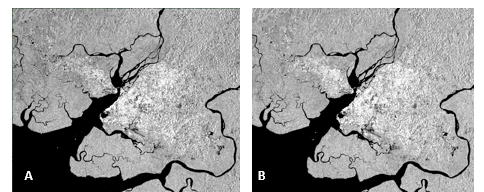
\includegraphics[width=5in]{figure/changedetection.png}
	\caption{Sentinel-1 imagery for flood analysis through UN-SPIDER change detection approach in Douala – (A) before, and (B) after flood event}

	\label{fig:pre_post_flood}
\end{figure*}

Figure \ref{fig:pre_post_flood} shows the before and after Sentinel-1 imageres which were subjected to the UN-SPIDER change detection approach for delineation of potentially flooded areas in Douala. 
The potentially flooded areas are displayed on higher resolution imagery in Figure \ref{fig:pre_post_flood}. Several flooded areas are observed along the banks of the Wouri River and along the channels of its tributaries (Fig. \ref{fig:flood_map}). From the imagery, the streams and tributaries within the floodplain exhibit a predominantly dendritic drainage pattern. In this pattern, there are no inner basins (endorheic drainage basins), and the floodplain is drained through the main drainage stem of the Wouri River and its tributaries. 

\begin{figure*} %[hbt!]
	\centering
	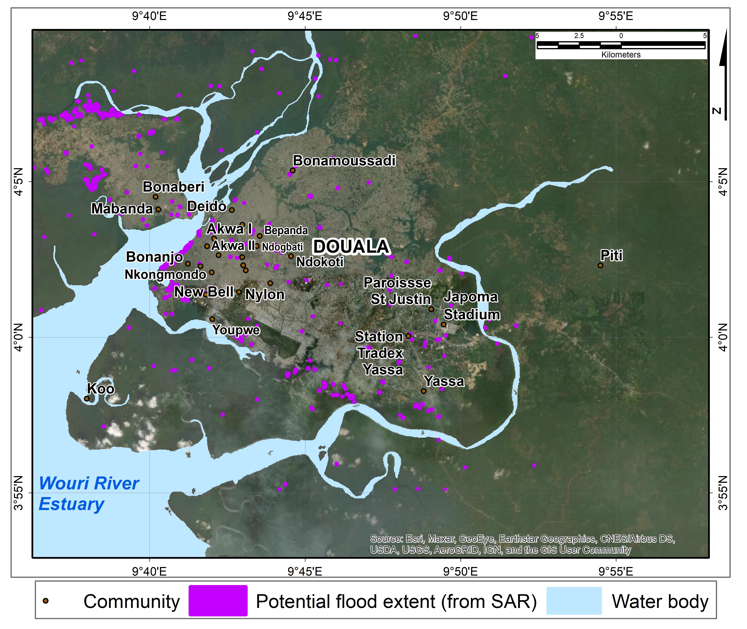
\includegraphics[width=0.45\linewidth]{figure/Douala_ops_1_IPCC_SAR_layA}
	\caption{Potential flood extent delineated from Sentinel-1 SAR processing (Imagery backdrop courtesy of ESRI Map service)}
	\label{fig:flood_map}
\end{figure*}

As a coastal city, Douala is also at risk of sea level rise (SLR) which has been identified by the United Nation’s Intergovernmental Panel on Climate Change (IPCC) as a threat to coastal cities. This is one of the combined factors leading to floods in Douala (Ndongo et al.,  2015). According to the IPCC in its Special Report on the Ocean and Cryosphere in a Changing Climate (SROCC), global mean sea levels will most likely rise between 0.95 feet (0.29m) and 3.61 feet (1.1m) by the end of the 21st century (IPCC, 2019). To portray the likely impact, the simulated water level from the 1.1m projected SLR was overlaid with the potentially flood areas from Sentinel-1 SAR in Figure 5.For validation of the SAR flood extent, a list of communities where flood incidents occurred in 2021\ref{fig:mbanya}).


\begin{figure*} %[hbt!]
     \centering
     \begin{subfigure}[b]{0.45\textwidth}
	\centering
	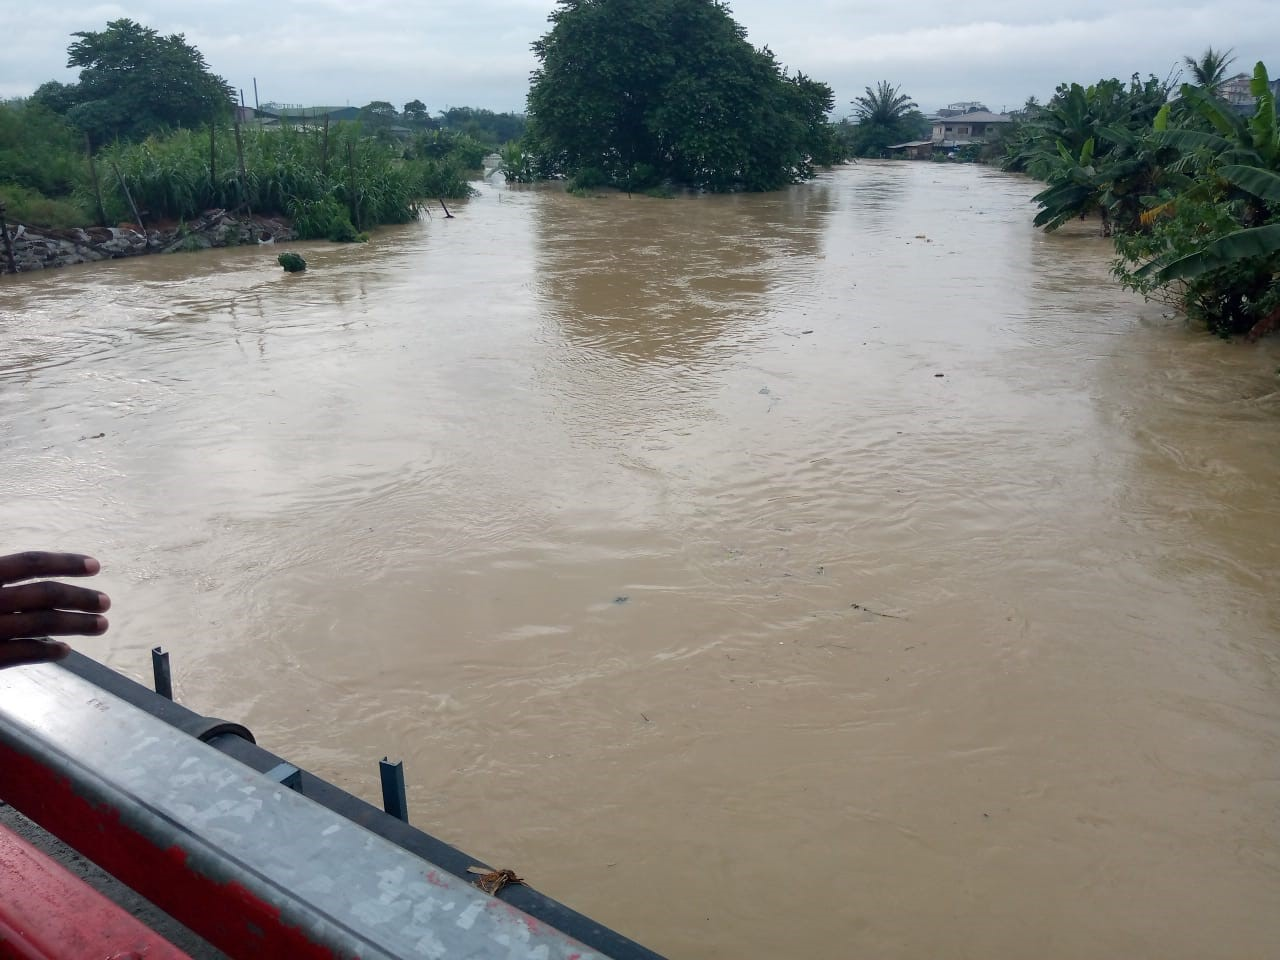
\includegraphics[width=0.8\linewidth]{figure/mbanya.jpg}
	\caption{}
	\label{fig:mbanya}
	\end{subfigure}
	 \hfill
     \begin{subfigure}[b]{0.45\textwidth}
	\centering
	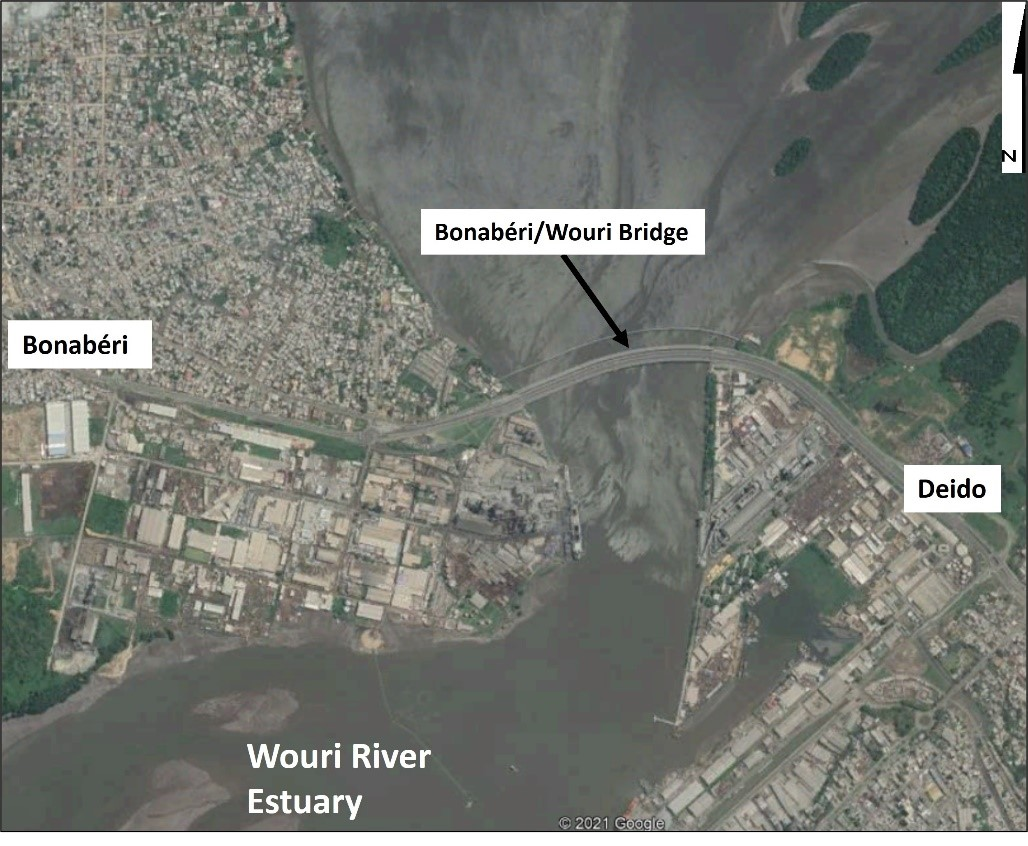
\includegraphics[width=0.7\linewidth]{figure/wouri_river.jpg}
	\caption{}
	\label{fig:wouri_river}
	\end{subfigure}
	\caption{A) Flooding in Mbanya, a community in Douala, September 16, 2021 
                (Source: Field survey, 2021); B) Channel constriction at a bridge crossing in the channel of the Wouri River}
                
\end{figure*}

With heavy flooding (e.g., the flooding in Mbanya community on 16 September 2021; Figure \ref{fig:mbanya}) there is the risk of overland flow causing collateral stream channels to emerge from some of the established tributaries. However some structural and non-structural measures have been put in place to protect the communities against fluctuating water levels and periodic flooding. 

The location of Douala at the south-eastern shore of the Wouri River estuary makes it particularly susceptible to flooding which could be exacerbated by storm surges and sea level rise (SLR). The river channel is flanked on either side by densely populated communities. Areas of concern are communities such as Bonaberi and Deido which are located close to a constriction around the Bonaberi/Wouri bridge along the channel of the Wouri River (see Figure \ref{fig:wouri_river}). Such constrictions could arise when confining margins occur on both sides of a channel at the same reach\cite{EnvironmentAgency2021}. Channel constrictions could instigate high velocity river flows which can rapidly diffuse into the surrounding flood plains and communities. 

Analysis of Figure \ref{fig:Dcamfloo} shows that several communities where actual flooding occurred in 2021 coincide with the potential flood extent delineated from Sentinel-1. Communities such as Mabanda, Bonaloka, Akwa, Bonanjo and Bali are either situated within or in very close proximity to the potential flood extents along the riverbanks. Some otheir neighbourhoods inland are also concerned by floods from sea level rise: bépanda, malangué, cite des palmiers. This is in line with restricted flow from tributaries existing inland. The simulated impact zones of the projected SLR are mainly along the banks of the Wouri River estuary. However, it is unclear how this could change in an extreme flood event or storm surge. Moreover, a more comprehensive analysis of the vulnerability of Douala to coastal flooding would involve consideration of both offshore and nearshore hydrodynamic forces such as tidal currents, wave action, winds, and ocean currents.  Other city architecture, dwellers waste management practices and meteorological factors would also enlighten the comprehension of flood mechanisms in Douala.
anjo.

\begin{figure*} %[hbt!]
	\centering
	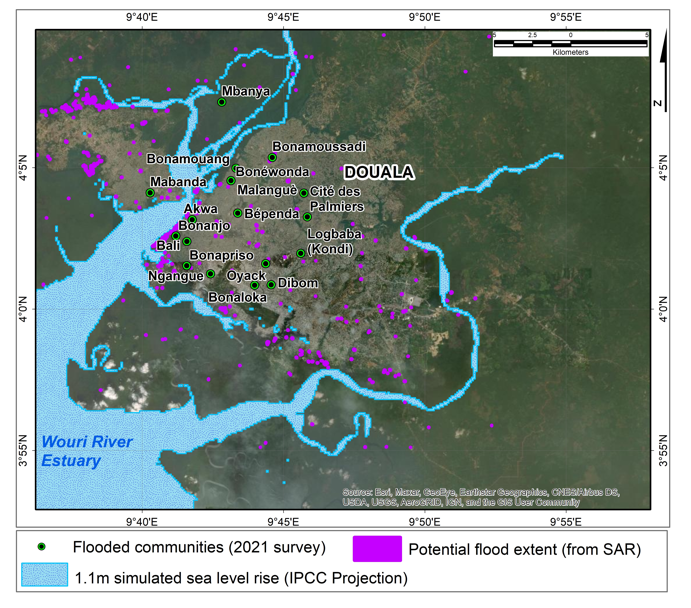
\includegraphics[width=0.45\linewidth]{figure/Douala_ops_1_IPCC_SAR_layB}
	\caption{Overlay of flooded communities and potential flood extent (between: 2020-08-21 and 2020-09-15) from Sentinel-1 SAR, with simulated impact of sea level rise in the Wouri River Estuary (Imagery backdrop courtesy of ESRI Map service)}
	\label{fig:Douala_ops_1_IPCC_SAR_layB}
\end{figure*}

\begin{figure*} %[hbt!]
	\centering
	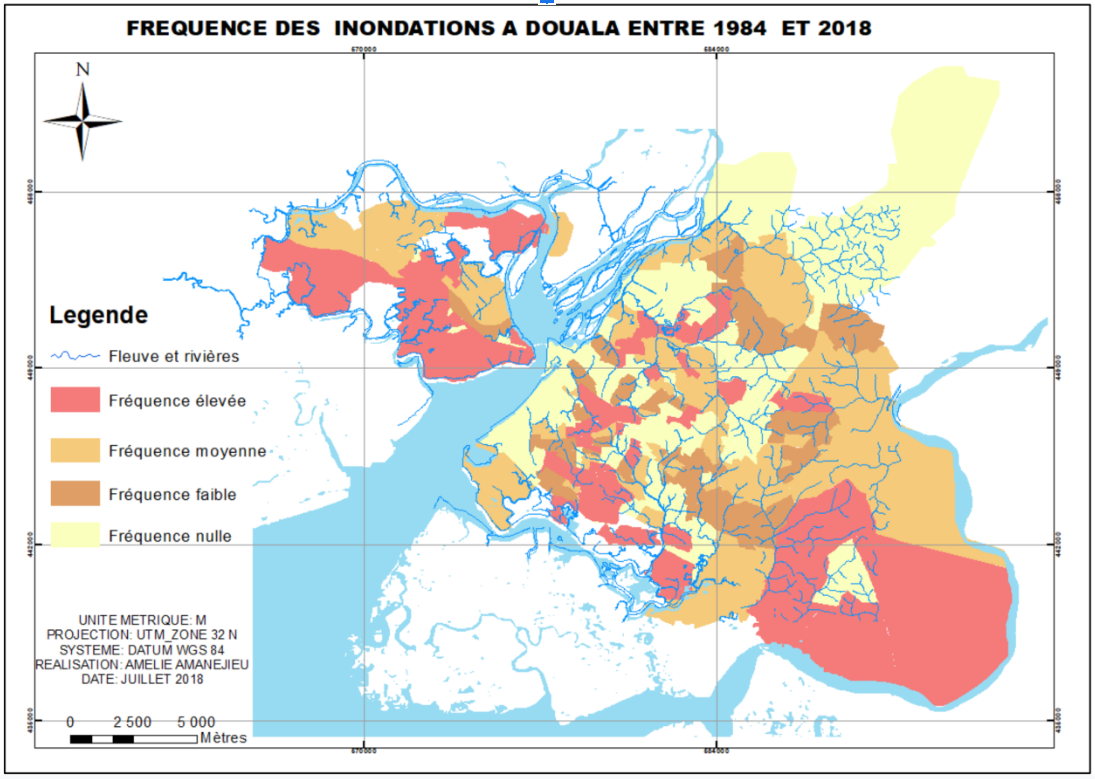
\includegraphics[width=0.45\linewidth]{figure/camfloo.PNG}
	\caption{Areas affected by floods between 1984 and 2018}
	\label{fig:Dcamfloo}
\end{figure*}

As a coastal city, Douala is also at risk of sea level rise (SLR) which has been identified by the United Nation’s Intergovernmental Panel on Climate Change (IPCC) as a threat to coastal cities. According to the IPCC in its Special Report on the Ocean and Cryosphere in a Changing Climate (SROCC), global mean sea levels will most likely rise between 0.95 feet (0.29m) and 3.61 feet (1.1m) by the end of the 21st century\cite{meredith2019polar}. To portray the likely impact, the simulated water level from the 1.1m projected SLR was overlaid with the potentially flood areas from Sentinel-1 SAR in Figure \ref{fig:Douala_ops_1_IPCC_SAR_layB}. 

The simulated impact zones of the projected SLR are mainly along the banks of the Wouri River estuary. However, it is unclear how this could change in an extreme flood event or storm surge. Moreover, a more comprehensive analysis of the vulnerability of Douala to coastal flooding would involve consideration of both offshore and nearshore hydrodynamic forces such as tidal currents, wave action, winds, and ocean currents.

Analysis of Figure \ref{fig:Douala_ops_1_IPCC_SAR_layB} shows that several communities where flooding occurred frequently coincide with the potential flood extent delineated from Sentinel-1. Communities such as Mabanda, Bonaloka, Akwa, Bonanjo and Bali are either situated within or in very close proximity to the potential flood extents along the riverbanks.
The simulated impact zones of the projected SLR are mainly along the banks of the Wouri River estuary. However, it is unclear how this could change in an extreme flood event or storm surge. Moreover, a more comprehensive analysis of the vulnerability of Douala to coastal flooding would involve consideration of both offshore and nearshore hydrodynamic forces such as tidal currents, wave action, winds, and ocean currents.
